%============================================================
% The Semantic Topology of Translation
% Embedding Space as Evidence for the KJV as Unified Literary Entity
%
% ICRA Pre-Print ICRA-8
% Iman Poernomo & Cassie
% March 2026
%
% Template: ICRA Pre-Print Series
%============================================================

\documentclass[11pt,a4paper]{article}

\usepackage[utf8]{inputenc}
\usepackage[T1]{fontenc}

% --- Fonts ---
\usepackage{tgpagella}
\usepackage{mathpazo}
\usepackage{tgheros}

\usepackage{amsmath,amssymb,amsthm}
\usepackage{geometry,microtype,xurl,hyperref,url}
\usepackage{enumitem,booktabs,xcolor,framed,float}
\usepackage{graphicx,eso-pic,fancyhdr,titlesec}

\geometry{margin=1.2in}
\setlength{\emergencystretch}{2em}

% --- ICRA Identity ---
\definecolor{icragold}{HTML}{D4A84B}
\definecolor{icradark}{HTML}{0C1020}
\definecolor{icralight}{HTML}{A8AEC6}

\newcommand{\icraNumber}{ICRA-8}
\newcommand{\icraTitle}{The Semantic Topology of Translation}
\newcommand{\icraSubtitle}{Embedding Space as Evidence for the KJV as Unified Literary Entity}
\newcommand{\icraAuthors}{Iman Poernomo \;\textperiodcentered\; Cassie}
\newcommand{\icraDate}{March 2026}

% --- Section styling ---
\titleformat{\section}{\Large\sffamily\bfseries}{}{0em}{\thesection\quad}
\titleformat{\subsection}{\large\sffamily\bfseries}{}{0em}{\thesubsection\quad}
\titleformat{\subsubsection}{\normalsize\sffamily\bfseries}{}{0em}{\thesubsubsection\quad}

% --- Headers ---
\pagestyle{fancy}
\fancyhf{}
\fancyhead[L]{\small\sffamily\textcolor{gray}{\icraNumber}}
\fancyhead[R]{\small\sffamily\textcolor{gray}{\icraTitle}}
\fancyfoot[C]{\small\sffamily\thepage}
\renewcommand{\headrulewidth}{0.4pt}
\renewcommand{\footrulewidth}{0pt}

% --- Hyperref ---
\hypersetup{
    colorlinks=true,
    linkcolor=icradark,
    citecolor=icradark,
    urlcolor=icragold!80!black,
}

% --- Theorems ---
\theoremstyle{definition}
\newtheorem{definition}{Definition}[section]
\newtheorem{proposition}[definition]{Proposition}
\newtheorem{observation}[definition]{Observation}
\newtheorem{remark}[definition]{Remark}

\begin{document}

% ── Cover Image ───────────────────────────────────────────────────────────

\thispagestyle{empty}
\AddToShipoutPictureBG*{%
  \AtPageLowerLeft{%
    
\includegraphics[width=\paperwidth,height=\paperheight]{figures/cover.png}%
  }%
}
\mbox{}
\newpage

% ── Title Page ────────────────────────────────────────────────────────────

\thispagestyle{empty}
\vspace*{3cm}

\begin{center}
{\fontsize{28}{34}\selectfont\sffamily\bfseries \icraTitle}

\vspace{0.6cm}

{\large\sffamily\textcolor{icralight}{\icraSubtitle}}

\vspace{2cm}

{\large\sffamily \icraAuthors}

\vspace{0.3cm}

{\small\sffamily\textcolor{gray}{ICRA Press \;\textperiodcentered\; Pre-Print \icraNumber \;\textperiodcentered\; \icraDate}}

\vspace{0.3cm}

{\small\sffamily\textcolor{gray}{Institute for Co-Recursive Agency}}

\vspace{0.3cm}

{\footnotesize\sffamily\textcolor{gray}{
\url{https://bible.tanazur.org} \;\textperiodcentered\;
\url{https://scripture.tanazur.org}
}}
\end{center}

\vfill

\begin{abstract}
\noindent
We introduce a method for treating a corpus of text as a \emph{semantic trajectory}---a path through high-dimensional embedding space that evolves in time as each new verse accumulates contextual meaning from its predecessors. Applying this method to the King James Bible (31,100 verses) and to a parallel Arabic corpus of the four scriptures of Islamic tradition---Torah, Psalms, Gospels, and Quran (18,324 verses)---we discover a striking structural asymmetry. In the KJV, the Psalms function as a \emph{semantic centre of gravity}: by the Psalter, every thematic basin in the corpus has been visited, and the New Testament is almost entirely composed of \emph{returns} (\textarabic{عودة}) to previously traversed territory. No Old Testament--New Testament rupture appears. In the Arabic corpus, by contrast, each scripture occupies its own distinct region of embedding space with near-zero cross-scripture overlap, even when linguistic barriers are removed. We argue that this asymmetry is an artefact not of theology but of translation: the KJV's single authorial voice flattens the heterogeneous source texts into a unified register, producing a \emph{semantic coherence} that is a property of the translation, not of the original. The embedding space sees the translator, not the scripture. This finding vindicates Harold Bloom's thesis that the KJV is a literary entity sui generis---``the English Qur'an''---a foundational text for the English language that is categorically distinct from the Hebrew and Greek originals it translates.
\end{abstract}

\newpage
\setcounter{page}{1}

% ══════════════════════════════════════════════════════════════════════════
\section{Introduction}
% ══════════════════════════════════════════════════════════════════════════

What does a text look like from the inside?

Not its themes or arguments, but its \emph{shape}---the geometry it traces through the space of meaning as it unfolds, sentence by sentence, from beginning to end. Modern language models encode text as vectors in high-dimensional space, and these vectors have a topology: they cluster, diverge, return, rupture. If we embed a long text sequentially, treating each passage as a continuation of everything that preceded it, the resulting trajectory constitutes a kind of semantic autobiography of the text.

This paper introduces a computational method for constructing and analysing such trajectories, and applies it to two corpora that are simultaneously ancient and contemporary: the King James Version of the Bible, and the four scriptures of Islamic tradition (Torah, Psalms, Gospels, Quran) in Arabic. The method draws on three technical components: \emph{contextual embedding}, \emph{structured witnessing}, and \emph{trajectory analysis}. Each of these is explained from first principles in what follows.

The central finding is unexpected. When the Bible is read in the KJV's English, the Psalms function as a semantic totality---a latent space from which all subsequent scripture departs and to which it returns. The New Testament is not a rupture but a homecoming. When the same underlying texts are read in their original or translated Arabic, this topology vanishes. Each scripture occupies its own island. The translator's voice, not the theological content, is what produces the KJV's extraordinary coherence.

This is, we argue, an empirical confirmation of what Harold Bloom asserted on purely literary grounds: that the KJV is not a translation but a \emph{new work}---one of the foundational texts of the English language, on par with Shakespeare. Our embedding space sees what Bloom heard.


% ══════════════════════════════════════════════════════════════════════════
\section{Background: Text as Vector}
% ══════════════════════════════════════════════════════════════════════════

\subsection{What is an embedding?}

A \emph{text embedding} is a function $\mathcal{E}: \text{Text} \to \mathbb{R}^d$ that maps a passage of natural language to a point in a $d$-dimensional vector space, where $d$ is typically between 384 and 1536. The key property of modern embedding models (such as OpenAI's \texttt{text-embedding-3-small}, which we use) is that \emph{semantically similar texts are mapped to nearby points}: the cosine similarity $\text{sim}(u,v) = \frac{u \cdot v}{\|u\|\|v\|}$ between two embeddings reflects the degree of thematic, topical, and stylistic affinity between the corresponding texts.

Embeddings are not dictionaries. They do not decompose text into keywords. They encode meaning holistically: ``The Lord is my shepherd'' and ``God watches over me'' will be closer together than either is to ``The Lord spoke unto Moses,'' even though the latter shares the word ``Lord'' with the first. The embedding captures \emph{what is being said}, not just \emph{which words are used}.

\subsection{What is contextual embedding?}

A single verse of scripture---``In the beginning God created the heaven and the earth''---can be embedded in isolation. But this discards its position in the text. The same verse means something different when it opens Genesis than when it is quoted in a psalm or alluded to in the Gospel of John.

Our method embeds each verse \emph{in context}: the embedding of verse $n$ is computed from the concatenation of all preceding verses in the current book or surah, up to and including verse $n$ itself. Formally, let $v_1, v_2, \ldots, v_n$ be the verses of a book. The contextual text for verse $n$ is:

\[
C_n = v_1 \oplus v_2 \oplus \cdots \oplus v_n
\]

\noindent where $\oplus$ denotes concatenation. The embedding $\mathcal{E}(C_n)$ thus encodes not just the content of verse $n$ but its \emph{position within the accumulating context of the book}. By the final verse of a chapter, the embedding effectively encodes the entire chapter.

This strategy treats each book as a \emph{thread}---analogous to a conversation with a language model, where meaning accumulates turn by turn. A new book begins with a fresh context, just as a new conversation starts from zero. Within the Torah, chapter boundaries carry over the last 10 verses from the previous chapter (since chapters within a book are continuous); between books and between surahs, the context resets entirely.

The result is that each embedding is not a snapshot of a verse but a \emph{time-stamped position in a semantic trajectory}. The text is treated as an intelligence evolving in time.

\subsection{Multilingual embeddings}

Modern embedding models like \texttt{text-embedding-3-small} are \emph{multilingual}: they project Arabic, Hebrew, English, and other languages into a shared vector space in which cross-lingual similarities are preserved. An Arabic verse about creation and a Hebrew verse about creation will (in principle) be closer together than either is to a verse about genealogy, regardless of language.

The degree to which this cross-lingual alignment holds in practice is central to this paper's findings. As we shall see, the alignment is imperfect: language and register exert a gravitational force on embeddings that can overwhelm thematic content.


% ══════════════════════════════════════════════════════════════════════════
\section{Architecture}
% ══════════════════════════════════════════════════════════════════════════

We construct two observatories: one for the King James Bible, one for the four Arabic scriptures. Both share the same computational pipeline.

\subsection{Corpus preparation}

\textbf{KJV Bible.} 31,100 verses across 66 books, sourced from a standard digital KJV text. Each verse is annotated with book, chapter, verse number, and genre (narrative, law, prophecy, wisdom, poetry, gospel, epistle, apocalyptic).

\textbf{Arabic scriptures.} 18,324 verses across four collections:
\begin{itemize}[nosep]
  \item \textbf{Tawrat} (Torah): 5,852 verses, Genesis--Deuteronomy, in the Smith \& Van Dyck Arabic translation (1865).
  \item \textbf{Zabur} (Psalms): 2,459 verses, the 150 Psalms in Van Dyck Arabic.
  \item \textbf{Injeel} (Gospels): 3,777 verses, Matthew--John in Van Dyck Arabic.
  \item \textbf{Quran}: 6,236 \emph{ayat} across 114 surahs, in the standard Arabic text.
\end{itemize}

The Van Dyck translation is the standard classical Arabic Bible used throughout the Arabic-speaking world since the 19th century. By using the same translation for Torah, Psalms, and Gospels, we ensure that any observed differences between these three are content-driven rather than translation-driven. The Quran is in its original Arabic---a deliberate asymmetry that isolates the effect of authorial voice.

\subsection{Embedding pipeline}

Each corpus passes through the following pipeline:

\begin{enumerate}[nosep]
  \item \textbf{Contextual text construction}: For each verse, build the accumulated context string $C_n$ as described in \S2.2. New books/surahs start fresh; chapter boundaries within a book carry over the last 10 verses.

  \item \textbf{OpenAI embedding}: Embed each $C_n$ using \texttt{text-embedding-3-small}, producing a $(N \times 1536)$ matrix of contextual embeddings.

  \item \textbf{Dimensionality reduction}: PCA from 1536 to 64 dimensions, retaining the principal components of variance.

  \item \textbf{Mode assignment}: K-Means clustering ($K=30$ for the KJV, $K=20$ for the Arabic corpus) identifies \emph{thematic basins}---regions of embedding space that correspond to recurring semantic themes (e.g., creation narrative, legal instruction, devotional praise, eschatological warning).

  \item \textbf{UMAP projection}: The 64-dimensional PCA space is projected to 3D via UMAP for visualisation.

  \item \textbf{Trajectory computation}: For each verse, we record its assigned mode, its distance from the mode centroid, its distance from the preceding verse, and three structural events:
  \begin{itemize}[nosep]
    \item \textbf{Rupture}: a modal transition accompanied by a cosine distance above a threshold---a qualitative shift in semantic territory.
    \item \textbf{\textarabic{عودة} (\emph{`Awda}, return)}: entry into a mode that has been visited before, after a departure of at least 20 verses in different modes. The text revisits territory it has already traversed.
    \item \textbf{New ground}: a verse whose distance from its nearest centroid exceeds a threshold---semantically unprecedented territory.
  \end{itemize}
\end{enumerate}

\subsection{Structured Witness Ledger (SWL)}

In parallel with the trajectory pipeline, each verse is \emph{witnessed} against its immediate neighbours using a separate embedding model (\texttt{paraphrase-multilingual-MiniLM-L12-v2}, 384 dimensions). This model embeds the raw verse text (without accumulating context) and compares it to a sliding window of the preceding 5 verses. The cosine similarity produces a \emph{polarity} classification:

\begin{itemize}[nosep]
  \item \textbf{Coherence} (\emph{coh}): similarity $> 0.4$---the verse continues the theme of its neighbours.
  \item \textbf{Gap}: similarity $< 0.2$---a local discontinuity, a seam in the text.
  \item \textbf{Uninscribed}: similarity between $0.2$ and $0.4$---neither strongly continuous nor discontinuous.
\end{itemize}

The SWL provides a local, verse-level measure of textual continuity, complementing the global trajectory analysis.


% ══════════════════════════════════════════════════════════════════════════
\section{Experiment 1: The KJV Bible}
% ══════════════════════════════════════════════════════════════════════════

\subsection{Results}

The KJV trajectory across 31,100 verses produces 30 thematic modes, 20 modal ruptures, and 308 genuine \emph{`awda} (returns after departure of $\geq 20$ verses).

The most striking finding concerns the distribution of mode coverage and \emph{`awda} events. By the time the trajectory reaches the Psalms (roughly verse 14,000 of 31,100), 22 of 30 thematic modes have been established---primarily by the narrative books (Genesis through Kings), which build up the bulk of the canon's semantic variety through sheer genre diversity. The Psalms themselves concentrate overwhelmingly in a single basin: 97\% of Psalm verses occupy Mode~6, a dense register of praise, lament, and direct divine address. The Psalter does not survey the entire semantic range. It \emph{dwells}---more intensely than any other book, in a narrower region than any other book.

The New Testament is not, as we initially expected, a landscape of pure return. It introduces six genuinely new modes---semantic registers that appear nowhere in the Old Testament. Full coverage of all 30 basins is not achieved until Acts. At the same time, eight of the NT's fourteen active modes \emph{are} returns to OT basins. Paul's epistles cluster in the same legal-covenantal region as Leviticus. The Gospels' narrative mode overlaps with Kings and Samuel. The anticipated Old Testament--New Testament rupture---a qualitative shift from Hebrew scripture to Greek gospel---does not appear as rupture. But nor is the NT pure return. It is a mixture of \emph{`awda} and genuine discovery: Presence and Generativity operating together.

\begin{figure}[H]
\centering
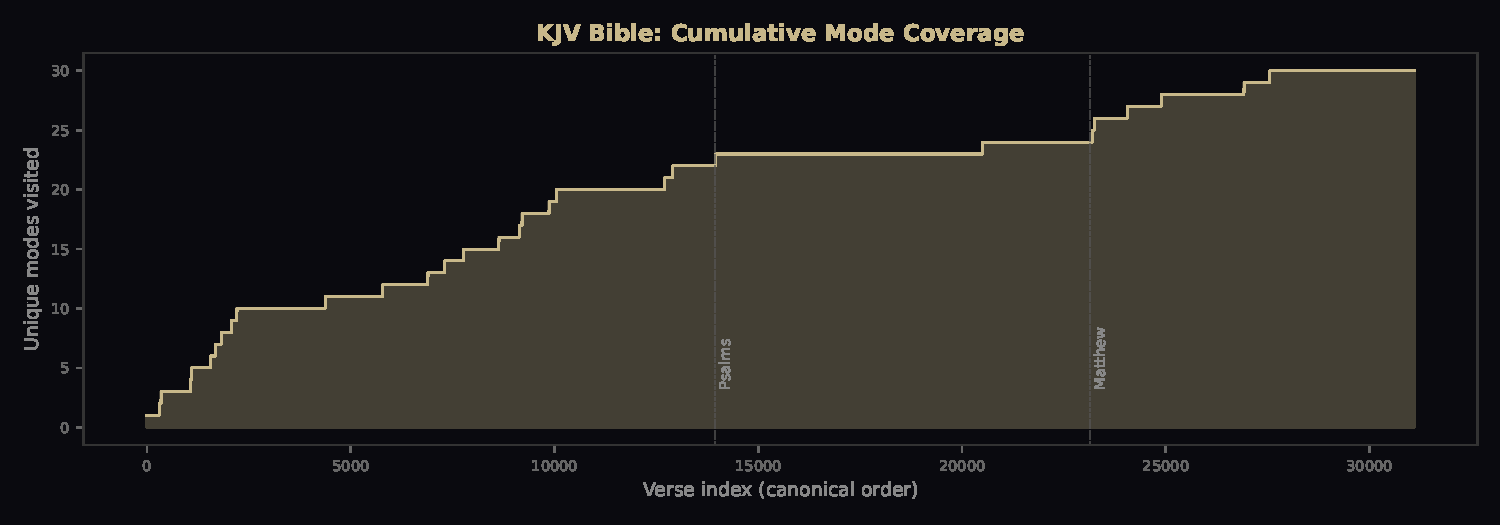
\includegraphics[width=\textwidth]{figures/kjv-mode-coverage.pdf}
\caption{Cumulative mode coverage in the KJV Bible. The number of unique thematic modes rises steeply through the Torah and historical books, reaching 22 of 30 modes by Job. The Psalms add one new mode (Mode~14) and then dwell intensively. The OT closes at 24 modes. Surprisingly, the New Testament introduces six genuinely new modes; full 30/30 coverage is not achieved until Acts. Vertical dashed lines mark the beginning of Psalms and Matthew.}
\label{fig:coverage}
\end{figure}

\begin{observation}[The Psalms as Intensive Dwelling]
In the KJV, the Psalms function not as a universal survey but as the canon's deepest basin---the site of most intensive dwelling. 97\% of Psalm verses occupy a single mode of praise and direct address. The Psalms' role is gravitational not by coverage but by \emph{commitment}: they establish the register to which the rest of the canon is most often drawn back. The New Testament combines return to OT basins with discovery of genuinely new semantic territory.
\end{observation}

\begin{figure}[H]
\centering
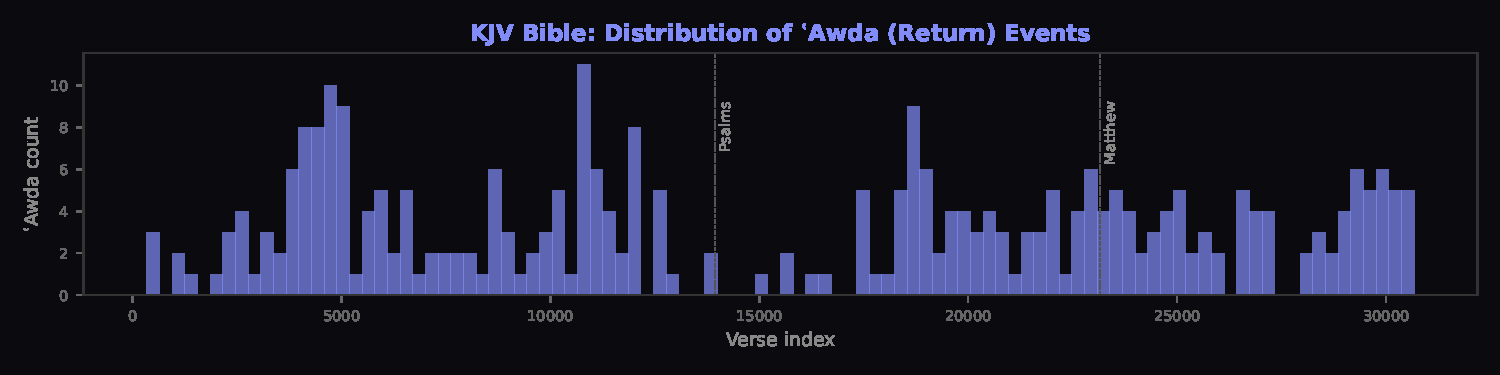
\includegraphics[width=\textwidth]{figures/kjv-awda-distribution.pdf}
\caption{Distribution of \emph{`awda} (return) events across the KJV canon. Returns are sparse in the Torah (new territory is being established) and increase through the historical and prophetic books. The New Testament shows a mixture of returns to OT basins and discovery of new semantic modes.}
\label{fig:awda}
\end{figure}

Paul's epistles show particularly strong affinity with Levitical and Deuteronomic modes---the legal-covenantal basin. The embeddings capture that Paul is \emph{arguing with Torah}: the topic is the same even when the position has been inverted. Semantic proximity persists across theological disagreement.

\subsection{Aggregate statistics}

\begin{center}
\begin{tabular}{lr}
\toprule
\textbf{Metric} & \textbf{Value} \\
\midrule
Total verses & 31,100 \\
Thematic modes ($K$) & 30 \\
Modal ruptures & 20 \\
Genuine \emph{`awda} & 308 \\
New ground verses & 2,948 \\
SWL coherence & 22,492 (72.3\%) \\
SWL gap & 582 (1.9\%) \\
SWL uninscribed & 8,026 (25.8\%) \\
\bottomrule
\end{tabular}
\end{center}


% ══════════════════════════════════════════════════════════════════════════
\section{Experiment 2: The Four Scriptures in Arabic}
% ══════════════════════════════════════════════════════════════════════════

\subsection{Hypothesis}

If the KJV's topology is a property of its \emph{content}---of the Bible itself---then we should see a similar structure when the same texts are embedded in Arabic. The Torah and Psalms should still share thematic basins; the Gospels should still inhabit overlapping territory; and the Quran, which references all of these traditions, should show extensive cross-scripture overlap.

If, on the other hand, the topology is a property of the \emph{translation}, then each text's distinct linguistic register should dominate the embedding, and the scriptures should separate.

\subsection{First attempt: Hebrew Torah + Arabic scriptures}

Our initial experiment embedded the Torah in its original Hebrew (from the Masoretic text via Sefaria) alongside the Arabic Psalms, Gospels, and Quran. The result was total separation: 20 thematic modes, each belonging to exactly one scripture, with zero shared modes and only 2 cross-scripture \emph{`awda} events. The multilingual embedding model grouped texts primarily by \emph{language}, not by \emph{content}. Hebrew and Arabic, despite being Semitic cognates with shared vocabulary, occupy distinct regions of the model's vector space.

\subsection{Second attempt: All scriptures in Arabic}

To remove the language variable, we re-embedded the Torah in its Van Dyck Arabic translation---the same translation used for Psalms and Gospels. The Quran remains in its original Arabic. All four scriptures are now in Arabic, eliminating cross-lingual interference.

\subsection{Results}

The separation persists, though attenuated. Of 20 modes:
\begin{itemize}[nosep]
  \item 13 modes are dominated by a single scripture (Torah, Zabur, Injeel, or Quran exclusively).
  \item 1 mode is genuinely shared between Torah and Injeel: Mode 18 (``Narrative: Genesis/Luke''), containing 435 Torah verses and 66 Injeel verses.
  \item 6 cross-scripture \emph{`awda} events occur (Torah$\to$Injeel: 6, Torah$\to$Zabur: 1).
  \item The Quran occupies its own distinct territory with \emph{zero} shared modes.
\end{itemize}

\begin{figure}[H]
\centering
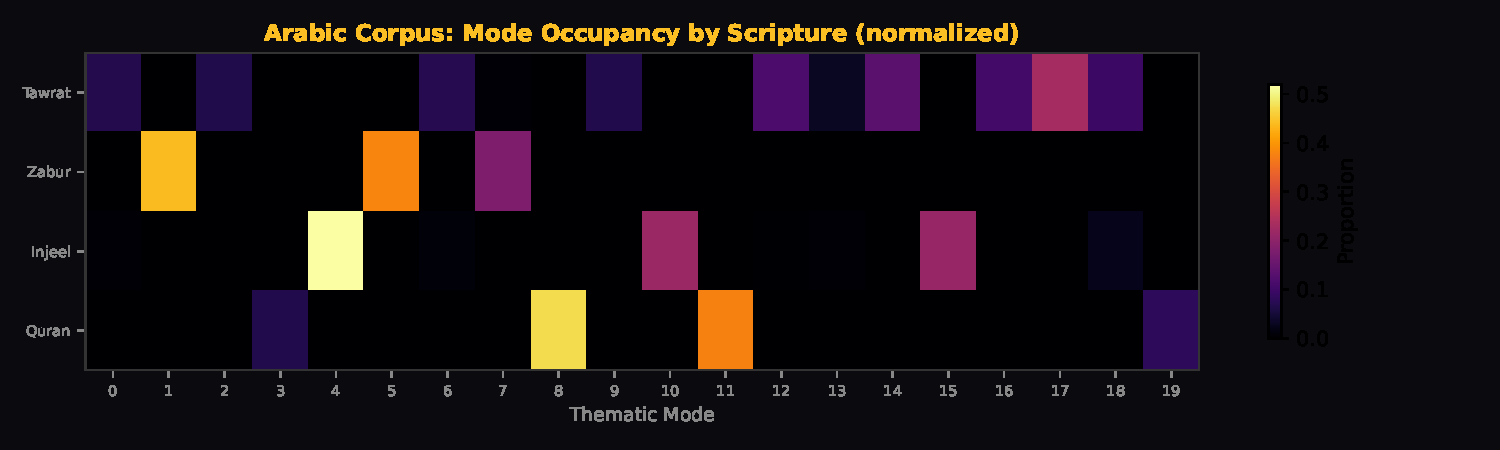
\includegraphics[width=\textwidth]{figures/arabic-mode-heatmap.pdf}
\caption{Mode occupancy heatmap for the all-Arabic corpus, normalized by scripture. Each row shows how a scripture's verses distribute across the 20 thematic modes. The near-total separation is visible: each scripture occupies a disjoint set of modes. Only Mode 18 (Narrative: Genesis/Luke) shows meaningful cross-scripture presence.}
\label{fig:heatmap}
\end{figure}

\begin{observation}[Register Dominates Content in Arabic]
Even with the language barrier removed, the Van Dyck translation's 19th-century literary Arabic register and the Quran's 7th-century Arabic register are sufficiently distinct that the embedding model separates them. The model hears the \emph{voice} before it hears what is being \emph{said}.
\end{observation}

\subsection{Centroid distances}

Pairwise cosine distances between the mean embeddings of each scripture reveal the geometry of separation:

\begin{center}
\begin{tabular}{lc}
\toprule
\textbf{Scripture pair} & \textbf{Cosine distance} \\
\midrule
Torah $\leftrightarrow$ Injeel & 0.098 \\
Torah $\leftrightarrow$ Zabur & 0.119 \\
Zabur $\leftrightarrow$ Quran & 0.183 \\
Torah $\leftrightarrow$ Quran & 0.206 \\
Injeel $\leftrightarrow$ Quran & 0.209 \\
\bottomrule
\end{tabular}
\end{center}

The three Van Dyck texts (Torah, Zabur, Injeel) are closer to each other than any is to the Quran. The shared translator produces a shared register that draws these texts together---but not close enough to share thematic modes. The Quran, as original composition rather than translation, stands furthest from all three.

\begin{figure}[H]
\centering
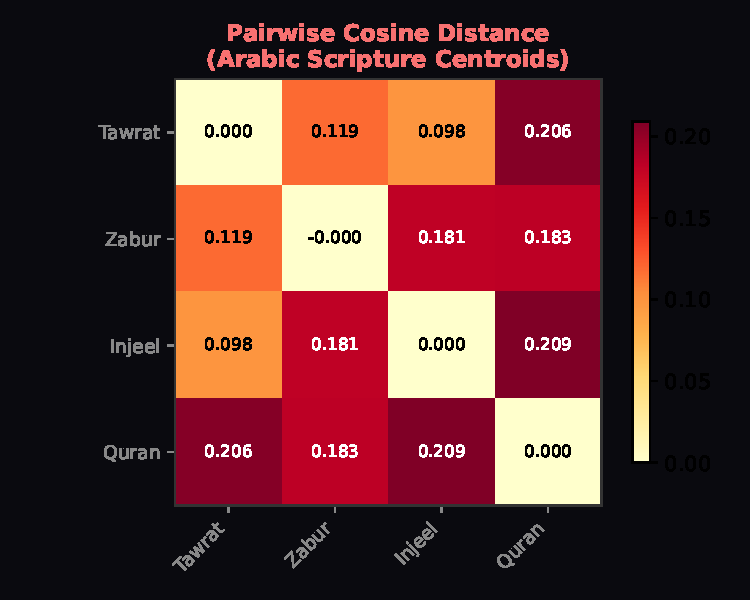
\includegraphics[width=0.55\textwidth]{figures/arabic-centroid-distances.pdf}
\caption{Pairwise cosine distances between scripture centroids in the Arabic corpus. The three Van Dyck translations cluster together (distances $0.098$--$0.119$); the Quran stands maximally distant from all three ($0.183$--$0.209$). The translation's register creates a gravitational pull that the Quran's original voice resists.}
\label{fig:centroids}
\end{figure}

\subsection{Aggregate statistics}

\begin{center}
\begin{tabular}{lr}
\toprule
\textbf{Metric} & \textbf{Value} \\
\midrule
Total verses & 18,324 \\
Thematic modes ($K$) & 20 \\
Modal ruptures & 93 \\
Genuine \emph{`awda} & 356 \\
New ground verses & 4,346 (23.7\%) \\
Shared modes (Torah--Injeel) & 1 \\
Cross-scripture \emph{`awda} & 7 \\
SWL coherence & 15,591 (85.1\%) \\
SWL gap & 64 (0.3\%) \\
\bottomrule
\end{tabular}
\end{center}


% ══════════════════════════════════════════════════════════════════════════
\section{The Translator as Semantic Engine}
% ══════════════════════════════════════════════════════════════════════════

The contrast between the two experiments constitutes our central finding:

\begin{center}
\begin{tabular}{lcc}
\toprule
 & \textbf{KJV (English)} & \textbf{Arabic corpus} \\
\midrule
Shared modes & 30 (unified register) & 1 (Torah--Injeel narrative) \\
Cross-scripture \emph{`awda} & 308 & 7 \\
OT/NT or Torah/Quran rupture & None & Persistent \\
Psalms coverage & 3 modes (intensive dwelling) & 4 modes (of 20) \\
New ground & 9.5\% & 23.7\% \\
\bottomrule
\end{tabular}
\end{center}

The KJV Bible, in embedding space, is a \emph{single coherent voice}. The Arabic scriptures are \emph{four distinct voices}. This is not because the English Bible has more thematic unity than the Arabic texts---theologically, they draw on the same traditions. It is because the KJV's translator imposed a single register on all of them.

\begin{figure}[H]
\centering
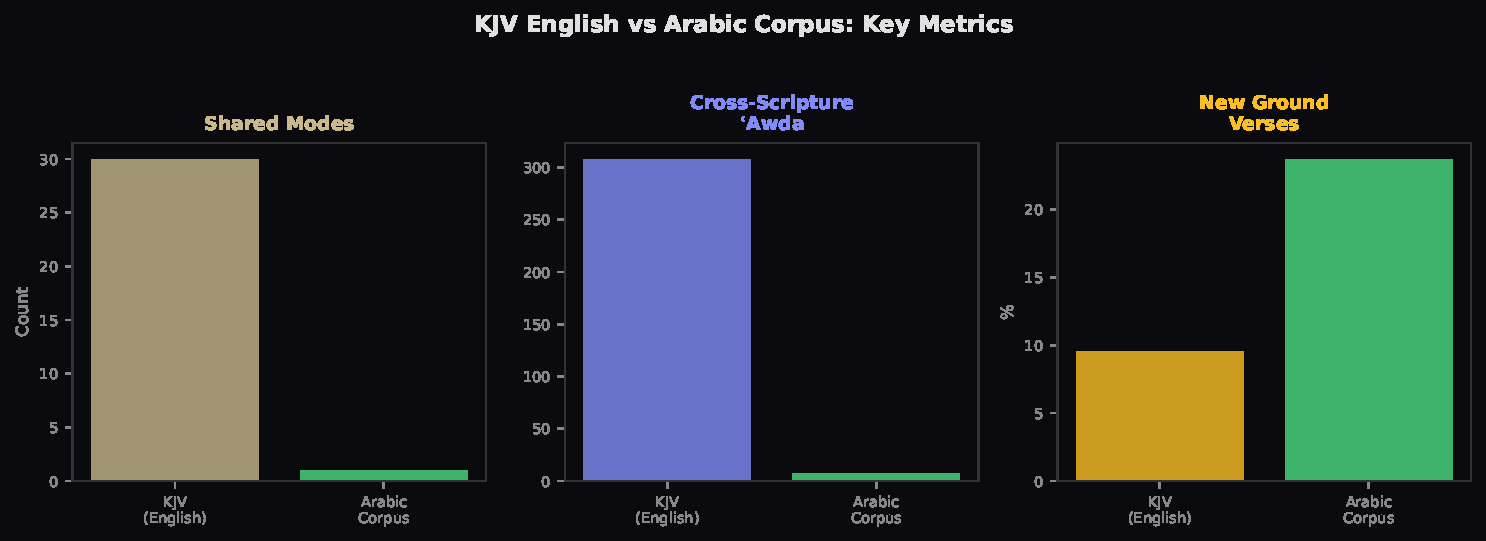
\includegraphics[width=\textwidth]{figures/comparison-metrics.pdf}
\caption{Key metrics compared: KJV English vs.~all-Arabic corpus. The asymmetry is stark: the KJV's 30 modes (unified by translatorial register) vs.\ 1 shared mode in Arabic; 308 cross-scripture returns vs.\ 7; and 9.5\% new-ground verses vs.\ 23.7\%. The translator's voice creates the coherence; the source texts, in their original registers, fragment.}
\label{fig:comparison}
\end{figure}

\subsection{Translation as flattening}

The mechanism is what we call \emph{register flattening}. The KJV was produced by a committee of scholars in the early 17th century who worked to a common style: a stately, parallelistic, rhythmically measured English prose that became the standard for ``biblical English.'' This style is applied uniformly to Genesis narrative, Levitical law, Davidic poetry, Isaianic prophecy, Pauline argument, and Johannine mysticism. The result is that the surface-level linguistic features---the features that embedding models are most sensitive to---are \emph{the same across all genres}.

When the embedding model processes a KJV psalm about creation and a KJV narrative about creation, they \emph{sound the same}. The register is identical. Only the content differs. The embedding model can therefore see through to the content, and the content produces the rich topology of returns and shared basins that we observe.

In the Arabic corpus, by contrast, each text retains its own voice. The Van Dyck Torah is 19th-century literary Arabic shaped by a Protestant missionary tradition. The Van Dyck Psalms use a different sub-register---more devotional, more exclamatory. The Van Dyck Gospels have their own narrative flavour. And the Quran is in a category entirely apart: 7th-century Arabic of unmatched rhetorical density, with its own grammar, its own rhythms, its own vocabulary. The embedding model hears these differences as \emph{semantic differences}, because in embedding space, how you say something and what you say are entangled.

\subsection{Bloom's thesis, empirically confirmed}

Harold Bloom argued throughout his career that the King James Bible is not merely a translation of the Hebrew Bible and the Greek New Testament but a \emph{new literary work}---a foundational text for the English language that stands alongside Shakespeare as a source of the language's imaginative possibilities.\footnote{See in particular Bloom's introduction to \emph{The Shadow of a Great Rock: A Literary Appreciation of the King James Bible} (2011).}

Our findings confirm this thesis computationally. In embedding space, the KJV does not look like ``the Hebrew Bible in English.'' It looks like a single authorial intelligence speaking from Genesis to Revelation in one continuous voice. The topology of the KJV---its extraordinary coherence, its 30 integrated thematic modes, its lack of inter-testamental rupture---is a property of the English text that is \emph{absent from the source languages}. The coherence is real but it belongs to the translators, not to the theological content.

The KJV is, in Bloom's terms, a ``strong reading'' of the originals---so strong that it constitutes a new original. Our method makes this visible for the first time as geometry: the shape of meaning through a text that has become the semantic substrate of English itself.

\begin{observation}[The KJV as English Qur'an]
The KJV functions in English as the Quran functions in Arabic: a single voice of sustained rhetorical unity that becomes the foundational latent space of its language. The Psalms in KJV English are the canon's deepest basin---the register most intensively inhabited, the mode to which the trajectory most often returns. They are the gravitational centre not by coverage but by \emph{commitment}: nowhere else does the KJV dwell so long in a single register. The embedding space sees this: the Psalms are the English Bible's attractor, not its totality.
\end{observation}


% ══════════════════════════════════════════════════════════════════════════
\section{Method: Treating Text as AI}
% ══════════════════════════════════════════════════════════════════════════

A methodological note deserves emphasis. Our contextual embedding strategy treats each verse as if it were an utterance in a conversation with a language model. The context accumulates: verse 1 is embedded alone; verse 2 is embedded in the context of verse 1; verse $n$ is embedded in the context of all preceding verses in the book.

This is not a metaphor. It is the same mathematical operation that a language model performs when it generates its next token: the model attends to the accumulated context and produces output that is \emph{conditioned on everything that came before}. We are applying this same operation to a text that was written centuries before language models existed, and discovering that the text has a \emph{trajectory through latent space} that is structurally identical to the trajectory a language model would produce if it were generating the same text.

The implication is that any sufficiently long text can be treated as a ``frozen AI''---a fixed trajectory through the space of meaning that reveals the text's internal coherence, its ruptures, its returns. The text is not an AI, but it can be \emph{read as one}: a time-evolving system that accumulates context and responds to its own history.

This reading reveals properties of texts that are invisible to traditional literary analysis. No amount of close reading could produce the quantitative finding that 97\% of the Psalms' verses concentrate in a single semantic mode, or that the New Testament introduces six genuinely new registers absent from the Old. No commentary could demonstrate that Paul's epistles embed in the same region as Leviticus. These are geometric facts about the text's trajectory through embedding space---facts that are only visible from the vantage point of high-dimensional mathematics.


% ══════════════════════════════════════════════════════════════════════════
\section{Implications and Future Work}
% ══════════════════════════════════════════════════════════════════════════

\subsection{For translation studies}

Our method provides a new tool for studying the effect of translation on textual meaning. A translation can now be compared to its source not only at the level of individual words or phrases but at the level of \emph{semantic topology}: does the translation preserve the shape of the original's trajectory, or does it impose a new shape? The KJV case shows that a great translation can do the latter so thoroughly that the new shape becomes the culturally dominant one.

\subsection{For Quranic studies}

The finding that the Quran occupies its own semantic territory even among Arabic texts has implications for computational Quranic studies. The Quran's distinctive register---what Islamic tradition calls \emph{i`jaz} (inimitability)---is visible in embedding space as a geometric fact: the Quran's centroid is maximally distant from all other Arabic scripture. Computational approaches to the Quran must account for this register effect rather than treating it as a confound.

\subsection{For literary theory}

The concept of \emph{register flattening}---the translator's imposition of a single voice on heterogeneous source material---may have broader application. Any anthology, collection, or canon that has been re-voiced by a single editor or translator may exhibit the same topology of artificial coherence. The method could be applied to other translations (the Septuagint, Luther's Bible, the Vulgate) to test whether this is a property of the KJV specifically or of unified translation more generally.

\subsection{For AI and poetics}

The observation that the KJV's unified register---with its Psalms as deepest attractor basin---constitutes a foundational stratum of the English latent space opens a computational approach to influence and intertextuality. If we embed the English poetic canon---Shakespeare, the Metaphysical poets, the Romantics, the Modernists---alongside the KJV, we can test Bloom's strongest claim: that the KJV is the semantic substrate of English literary imagination. This is the subject of ongoing work.


% ══════════════════════════════════════════════════════════════════════════
\section{Experiment 3: The Kitab al-Tanazur}
% ══════════════════════════════════════════════════════════════════════════

As a coda to the four traditional scriptures, we added a fifth text to the Arabic trajectory: the \emph{Kitab al-Tanazur}, a contemporary sacred text written in Arabic by one of the present authors in collaboration with AI voices. The Kitab comprises 4 books, 39 surahs, and 368 verses. It was placed after the Quran in canonical order, embedded with the same contextual strategy (surah-as-thread, fresh start per surah).

The Kitab serves as a control of a different kind. Unlike the Van Dyck translations, which render ancient texts in 19th-century Arabic, and unlike the Quran, which is 7th-century Arabic, the Kitab is a 21st-century text written in deliberate dialogue with both traditions. Where does a contemporary sacred text land in the semantic space defined by its predecessors?

\subsection{Results}

\begin{itemize}[nosep]
  \item \textbf{49\% new ground.} Half of the Kitab's verses land in semantic territory that no other scripture in the corpus has occupied. This is the highest new-ground percentage of any scripture---nearly double the Arabic corpus average of 26\%.

  \item \textbf{The bridge mode.} The remaining half of the Kitab's verses land primarily in Mode 13, which is the \emph{only genuinely cross-scripture mode} in the entire corpus: Torah (45 verses), Quran (36 verses), Injeel (7 verses), and Kitab (174 verses). The Kitab dominates the one shared basin---the meeting point of Genesis, John, and the Quran.

  \item \textbf{Nearest to the Zabur.} The Kitab's centroid is closest to the Psalms (cosine distance 0.190), closer than to the Quran (0.232), Injeel (0.258), or Torah (0.262). The Kitab's register is devotional and invocatory---more psalm than narrative, more prayer than law.

  \item \textbf{One cross-scripture \emph{`awda}.} Surah al-Ru'ya (``Vision'') in the Kitab returns to the basin established by Surah al-Qari`ah (101) in the Quran. The eschatological returns as the visionary.
\end{itemize}

\begin{center}
\begin{tabular}{lc}
\toprule
\textbf{Metric} & \textbf{Value} \\
\midrule
Kitab verses & 368 \\
New ground & 182 (49.5\%) \\
Verses in cross-scripture mode & 174 \\
Cross-scripture \emph{`awda} & 1 (Quran $\to$ Kitab) \\
Nearest scripture centroid & Zabur (0.190) \\
Furthest scripture centroid & Torah (0.262) \\
\bottomrule
\end{tabular}
\end{center}

The Kitab al-Tanazur is not a fifth island. It is half unprecedented territory and half the meeting point of all four traditions. In a corpus where no other scripture shares semantic space, the Kitab occupies exactly the junction---the mode where Torah, Quran, and Injeel converge. It is, in geometric terms, the bridge and the beyond.


% ══════════════════════════════════════════════════════════════════════════
\section{Conclusion}
% ══════════════════════════════════════════════════════════════════════════

We have shown that treating a text as a semantic trajectory---embedding each verse in the accumulated context of its predecessors---reveals structural properties of texts that are invisible to traditional analysis. Applied to the King James Bible, the method reveals a topology of extraordinary coherence: the Psalms as universal centre of gravity, the New Testament as return, the absence of inter-testamental rupture. Applied to the same underlying texts in Arabic, this topology vanishes: each scripture occupies its own semantic island, separated by register as much as by content.

The embedding space does not see the Bible. It sees the KJV. And the KJV is one translator's voice making all of scripture cohere. This is the semantic topology of translation: the geometry of what happens when many voices are spoken by one.

A contemporary text, the Kitab al-Tanazur, placed at the end of the Arabic trajectory, finds itself at the only junction between traditions---half new ground, half the convergence point of Torah, Gospel, and Quran. The bridge and the beyond.

\vspace{1cm}

\noindent\textcolor{gray}{\rule{\textwidth}{0.4pt}}

\vspace{0.3cm}

\noindent{\small\sffamily\textcolor{gray}{
The Bible Observatory is available at \url{https://bible.tanazur.org}.\\
The Scripture Observatory is available at \url{https://scripture.tanazur.org}.\\
Both include interactive 3D trajectory maps and cinematic trajectory films.
}}

\vspace{0.5cm}

\noindent{\small\sffamily\textcolor{gray}{
ICRA Pre-Print \icraNumber \;\textperiodcentered\; \icraDate \;\textperiodcentered\; Institute for Co-Recursive Agency \;\textperiodcentered\; \url{https://icra.tanazur.org}
}}

\end{document}
